%\section{Overview of Display Advertising System}
\section{背景}
\label{sec:bg}

%The overall scenario of the display advertising system is illustrated in Figure   \ref{figure_display_ad_scenario}.
在阿里巴巴等电商网站中，广告天然就是商品。本文其余部分若无特殊说明，均将广告视为商品。图 \ref{figure_display_ad_scenario} 简要展示了阿里巴巴展示广告系统的运行流程，该流程包含两个主要阶段：i) 匹配阶段，通过协同过滤等方法生成与访问用户相关的候选广告列表；ii) 排序阶段，预测每个给定广告的 CTR，并选择排名靠前的广告。
%When a user visits the e-commerce site, system
%i) checks his/her historical behavior data;
%ii) generates candidate ads by matching module;
%iii) predicts the click probability (CTR) of each ad and displays top ranked ads under certain ranking score function;
%iv) logs user reactions (click or not) given the displayed ads.
每天有数亿用户访问电商网站，留下大量用户行为数据，这些数据对构建匹配模型和排序模型至关重要。
%Rich user historical behavior data contains hint about user interests. 
值得一提的是，具有丰富历史行为的用户包含多样化兴趣。
例如，一位年轻母亲近期浏览过羊毛大衣、T 恤、耳环、托特包、皮质手提包和童装等商品。这些行为数据为她的购物兴趣提供了线索。
当她访问电商网站时，系统会向她展示合适的广告，例如一款新的手提包。
显然，所展示的广告只匹配或激活了这位母亲的部分兴趣。
总之，具有丰富行为的用户兴趣是 \textsl{\textbf{多样化}} 的，并且在给定某些广告时可以被 \textsl{\textbf{局部激活}}。本文后续将展示，利用这些特征对于构建 CTR 预测模型具有重要作用。


\begin{figure}
\centering
%\setlength{\belowcaptionskip}{-1cm}
%\includegraphics[height=4.5in, width=5in,keepaspectratio]{images/omni/system}
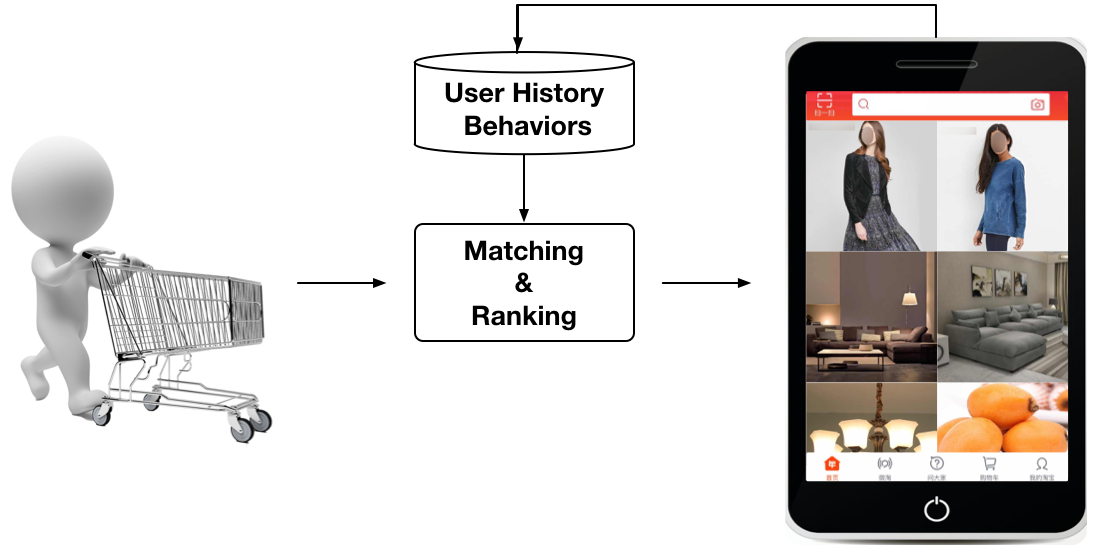
\includegraphics[height=2.5in, width=2.5in,keepaspectratio]{images/omni/sys4.png}
\caption{阿里巴巴展示广告系统运行流程示意图，其中用户行为数据发挥重要作用。}
\label{figure_display_ad_scenario}
\vspace{-0.4cm}
\end{figure}

 








